\documentclass[t,aspectratio=169]{beamer}

\usepackage{bm}
\usepackage{soul}
\usepackage{tikz}
\usepackage{tikz-3dplot}
\usepackage{amsmath}
\usepackage{amsfonts}
\usepackage{amssymb}
%\usepackage{physics}
%\usepackage{graphicx}
\usepackage{multicol}
\usepackage{t1enc}
\usepackage[utf8]{inputenc}
\usepackage[magyar]{babel}
\usepackage{pgfplots}
\pgfplotsset{compat=1.18}


\usetikzlibrary{calc,3d,decorations.pathmorphing,decorations.pathreplacing,decorations.markings,snakes,arrows.meta,calc,patterns}
\tikzset{snake it/.style={decorate, decoration=snake}}
% \usetheme{Madrid}
% \usecolortheme{whale}

%\usepackage{hyperref}
\hypersetup{
    colorlinks=true,
    linkcolor=blue,
    filecolor=magenta,      
    urlcolor=cyan,
    pdftitle={(KTXFI1EBNF) Physics I. Lecture},
}

% ----------------------------------------------------------------------------------------------------------------------------------------

\title{\includegraphics[width=45pt]{oepecsetlogo.png}\\(KTXFI1EBNF) Physics I. Lecture}

\author{Dr.~Gábor FACSKÓ, PhD\\\tiny Assistant Professor / Senior Research Fellow\\\textit{facsko.gabor@uni-obuda.hu}}

\institute{\Tiny Óbuda University, Faculty of Electrical Engineering, 1084 Budapest, Tavaszmező u. 17.\\Wigner Research Centre for Physics, Department of Space Physics and Space Technology, 1121 Budapest, Konkoly-Thege~Miklós~út~29–33.\\ \url{https://wigner.hu/~facsko.gabor}}

\date{April~13,~2026}

\logo{\includegraphics[height=0.9 true cm]{kekcsik.png}}

% ----------------------------------------------------------------------------------------------------------------------------------------

\begin{document}

\frame{\titlepage}

% ----------------------------------------------------------------------------------------------------------------------------------------

\begin{frame}
\frametitle{Current Updates and Announcements}
\begin{itemize}
\setlength{\parskip}{0pt}
\setlength{\itemsep}{4pt}
\item The exam dates and locations (rooms) have been finalized.
\item Opportunities to retake signatures will be available on May 26, 2026.
\item New mechanics exercises will be posted $\rightarrow$ Homework No.~4 and~5.
\end{itemize}
\end{frame}


% ----------------------------------------------------------------------------------------------------------------------------------------

\begin{frame}[fragile,squeeze,allowframebreaks]
\frametitle{Where are we?}
\begin{enumerate}
\setlength{\parskip}{0pt}
\setlength{\itemsep}{0pt}
\item \textbf{Mechanics I.:} Newton’s laws, equation of motion (review). Momentum. General concept of mechanical work, work theorem. Forms of mechanical energy.
\item \textbf{Mechanics II.:} Weight force, gravitational force, gravitational field. Work of the gravitational force. Conservative force field. Dissipative force field. Mechanical power.
\item \textbf{Mechanics of Rigid Bodies I.} Concept of a rigid body. Forces acting on a rigid body. Motion of a rigid body. Concept of the centre of mass. Location of the centre of mass. Torque. Angular momentum. Energy of a rotating rigid body, angular momentum of a rotating rigid body, Steiner’s theorem.
\item \textbf{Mechanics of Rigid Bodies II.} Principal theorems of rigid body motion; conservation laws. Collisions.
\item \textbf{Oscillations I.} Dynamic condition of harmonic oscillatory motion. Differential equation of harmonic undamped oscillatory motion.
\pagebreak
\item \textbf{Oscillations II.} Superposition of oscillations. Decomposition of oscillations into components. Damped oscillations. Forced oscillations, resonance. Coupled oscillations.
\item \textbf{Wave phenomena:} Reflection of waves, refraction of waves, diffraction of waves. Huygens–Fresnel principle. Interference of waves. Polarization of waves.
\item \textbf{Elements of acoustics:} Basics of acoustics. Fundamental concepts. Doppler effect. Sound intensity, loudness according to Weber–Fechner’s law.
\item \textbf{Thermodynamics I:} Temperature scales, thermal expansion, thermometers. State variables, ideal gas, state changes, ideal gas equation of state, Boyle’s law, Gay-Lussac’s laws, universal (combined) gas law, heat, specific heat, molar heat, heat capacity.
\item \textbf{Thermodynamics II:} Expansion work, internal energy, the first law of thermodynamics, forms of the first law in different state changes.
\pagebreak
\vskip -10 pt
\item \textbf{Thermodynamics III:} Cyclic processes, Carnot cycle, Carnot’s theorem, reduced heat, entropy, the second law of thermodynamics.
\item \textbf{Thermodynamics IV:} Kinetic theory of gases, molecular thermodynamics. Distributions, distribution functions. Elementary statistics.
\item \textbf{Electrostatics I.:} \textit{Electric charge: Fundamental electrical phenomena, electric charge and matter, Coulomb’s law (force between two point charges, unit of electric charge, permittivity of vacuum).}
\item \textbf{Electrostatics II.:} \textit{The electric field: The electrostatic field (electric field strength, electric field lines). Determination of electric field strength. Gauss’s law (flux of the electric field). Electric field of a point charge.}
\pagebreak
\item \textbf{Electrostatics III.:} Electrostatic potential: Work of the electric field (work done in an electric field). Electric potential (electrostatic potential). Electric potential difference, voltage. Electric potential of charge systems at small and large distances. Electrostatic energy.
\item \textbf{Elements of physical or wave optics.} Branches of optics. Light interference, light diffraction, diffraction through a slit, optical grating, light polarization. Light as an electromagnetic wave: Poynting vector. Optical instruments.
\end{enumerate}
\end{frame}

% ----------------------------------------------------------------------------------------------------------------------------------------

% Slide 1: Fundamental Electrical Phenomena
\begin{frame}[fragile,squeeze,allowframebreaks]
\frametitle{Fundamental Electrical Phenomena}
\begin{itemize}
\setlength{\parskip}{0pt}
\setlength{\itemsep}{4pt}
\item \textbf{Observation:} Certain materials, when rubbed together, exert forces on each other (electrostatics).
\item \textbf{Two types of charges:} Benjamin Franklin named them \textit{positive} and \textit{negative}.
\item \textbf{Basic Rule:} 
\begin{itemize}
\item Like charges \textbf{repel} each other.
\item Opposite charges \textbf{attract} each other.
\end{itemize}
\item \textbf{Conservation of Charge:} The total electric charge in an isolated system remains constant.

  \pagebreak

  
\item Electric Charge and Matter
    \begin{itemize}
        \item \textbf{Microscopic View:} Matter is composed of atoms.
        \begin{itemize}
            \item \textbf{Protons:} Positive charge (+e), located in the nucleus.
            \item \textbf{Electrons:} Negative charge (-e), orbiting the nucleus.
            \item \textbf{Neutrons:} Neutral (no charge).
        \end{itemize}
        \item \textbf{Quantization of Charge:} Charge exists only in discrete packets. 
        $$ q = n \cdot e $$
        where $e \approx 1.602 \times 10^{-19}$ C and $n$ is an integer.
        \item \textbf{Conductors vs. Insulators:} Conductors (like metals) allow charges to move freely; insulators do not.
        \end{itemize}

\pagebreak
\item Charge Distribution in Conductors with Cavities Why do charges move to the outer surface?
\vskip -20 pt
\begin{columns}

% LEFT COLUMN: FIGURE
  \begin{column}{0.4\textwidth}
\vfill
\centering
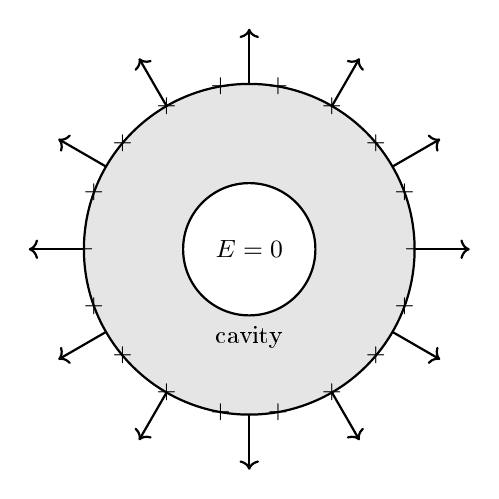
\begin{tikzpicture}[scale=0.7]

% Outer conductor
\fill[gray!20] (0,0) circle (3);

% Cavity
\fill[white] (0,0) circle (1.2);

% Boundaries
\draw[thick] (0,0) circle (3);
\draw[thick] (0,0) circle (1.2);

% Charges on outer surface
\foreach \angle in {0,20,...,340} {
\node at ({3*cos(\angle)}, {3*sin(\angle)}) {\small $+$};
}

% Electric field arrows outside
\foreach \angle in {0,30,...,330} {
\draw[->, thick]
({3*cos(\angle)}, {3*sin(\angle)}) --
({4*cos(\angle)}, {4*sin(\angle)});
}

% Labels
\node at (0,0) {\small $E = 0$};
\node at (0,-1.6) {\small cavity};

\end{tikzpicture}
\end{column}

% RIGHT COLUMN: TEXT
\begin{column}{0.6\textwidth}

\textbf{Electrostatic equilibrium:}
\begin{itemize}
\item The electric field inside a conductor must be zero.
\item Otherwise, free charges would move.
\end{itemize}

\textbf{Consequence:}
\begin{itemize}
\item Charges rearrange until the potential is constant.
\item The conductor becomes an equipotential body.
\end{itemize}

\textbf{Cavity:}
\begin{itemize}
\item If no charge is inside, then $E=0$ in the cavity.
\item No charge can remain in the bulk.
\end{itemize}
\end{column}

\end{columns}

\pagebreak
\item Physical intuition

\begin{columns}
\begin{column}{0.4\textwidth}

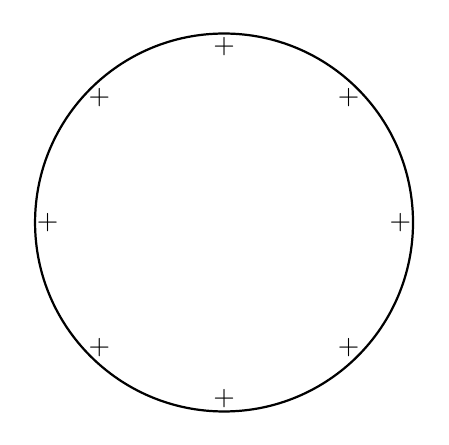
\begin{tikzpicture}[scale=0.8]

% Outer circle
\draw[thick] (0,0) circle (3);

% Charges spreading
\foreach \angle in {0,45,...,315} {
\node at ({2.8*cos(\angle)}, {2.8*sin(\angle)}) {$+$};
}

\end{tikzpicture}
\end{column}

\begin{column}{0.6\textwidth}

\textbf{Intuitive picture:}
\begin{itemize}
\item Charges repel each other.
\item They try to maximize their distance.
\item The outer surface provides the largest separation.
\end{itemize}

\textbf{Result:}
\begin{itemize}
\item Charges migrate outward.
\item Stable configuration: surface distribution.
\end{itemize}
\end{column}

\end{columns}

\pagebreak
\item Van de Graaff Generator: Principle of Operation

\begin{columns}

% LEFT: FIGURE
\begin{column}{0.3\textwidth}
\vfill
\centering
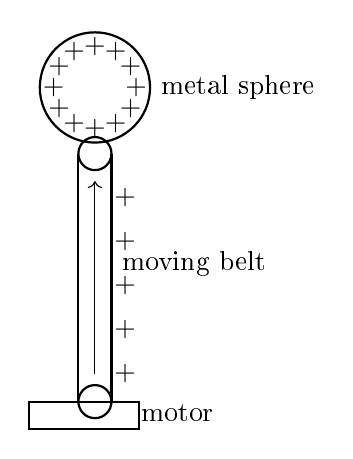
\begin{tikzpicture}[scale=0.7]

% Base
\draw[thick] (-1,-3) rectangle (1,-2.5);

% Belt
\draw[thick] (-0.1,-2.5) -- (-0.1,2);
\draw[thick] (0.5,-2.5) -- (0.5,2);

% Bottom roller
\draw[thick] (0.2,-2.5) circle (0.3);

% Top roller
\draw[thick] (0.2,2) circle (0.3);

% Sphere
\draw[thick] (0.2,3.2) circle (1);

% Arrows (belt motion)
\draw[->] (0.2,-2) -- (0.2,1.5);

% Charges on belt
\foreach \y in {-2,-1.2,-0.4,0.4,1.2} {
\node at (0.75,\y) {$+$};
}

% Charges on sphere
\foreach \angle in {0,30,...,330} {
\node at ({0.2+0.75*cos(\angle)}, {3.2+0.75*sin(\angle)}) {$+$};
}

% Labels
\node at (1.7,-2.7) {motor};
\node at (2.0,0) {moving belt};
\node at (2.8,3.2) {metal sphere};

\end{tikzpicture}
\end{column}

% RIGHT: TEXT
\begin{column}{0.5\textwidth}

\textbf{Basic idea:}
\begin{itemize}
\item A moving belt transports electric charge.
\item Charge is continuously deposited onto a metal sphere.
\end{itemize}

\textbf{Key property:}
\begin{itemize}
\item Charge accumulates on the outer surface.
\item Very high voltage can be reached.
\end{itemize}
\end{column}

\end{columns}

\pagebreak
\item Van de Graaff Generator: Charge Transport Mechanism

\begin{columns}

\begin{column}{0.3\textwidth}
\centering
\vfill
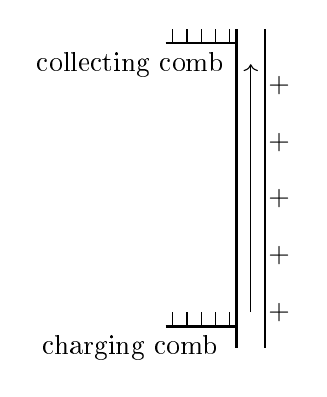
\begin{tikzpicture}[scale=0.9]

% Belt
\draw[thick] (0,-2.5) -- (0,2);
\draw[thick] (0.4,-2.5) -- (0.4,2);

% Bottom comb
\draw[thick] (-1,-2.2) -- (0,-2.2);
\foreach \x in {-0.9,-0.7,-0.5,-0.3,-0.1} {
\draw (\x,-2.2) -- (\x,-2);
}

% Top comb
\draw[thick] (-1,1.8) -- (0,1.8);
\foreach \x in {-0.9,-0.7,-0.5,-0.3,-0.1} {
\draw (\x,1.8) -- (\x,2);
}

% Charges moving up
\foreach \y in {-2,-1.2,-0.4,0.4,1.2} {
\node at (0.6,\y) {$+$};
}

% Arrow
\draw[->] (0.2,-2) -- (0.2,1.5);

\node at (-1.5,-2.5) {charging comb};
\node at (-1.5,1.5) {collecting comb};

\end{tikzpicture}
\end{column}

\begin{column}{0.65\textwidth}

\textbf{Steps:}
\begin{enumerate}
\item A high voltage source creates charge at the lower comb.
\item The belt picks up charge by corona discharge.
\item The belt carries charge upward.
\item At the top, charge is transferred to the sphere.
\end{enumerate}
\end{column}

\end{columns}


\pagebreak
\item Van de Graaff Generator: Why does voltage become very large?

\begin{columns}

\begin{column}{0.5\textwidth}
\vfill
\centering
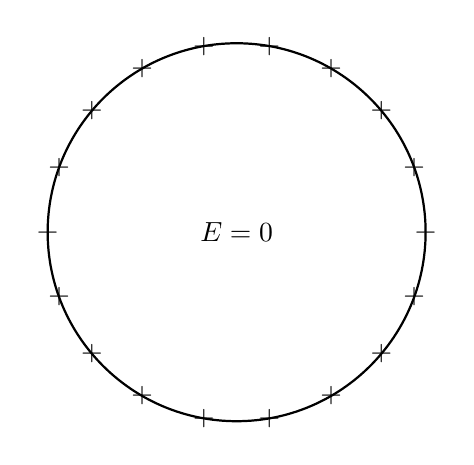
\begin{tikzpicture}[scale=1.2]

% Sphere
\draw[thick] (0,0) circle (2);

% Charges
\foreach \angle in {0,20,...,340} {
\node at ({2*cos(\angle)}, {2*sin(\angle)}) {$+$};
}

\node at (0,0) {$E=0$};

\end{tikzpicture}
\end{column}

\begin{column}{0.5\textwidth}
\textbf{Electrostatic properties:}
\begin{itemize}
\item Inside a conductor: $E = 0$.
\item Charge resides on the surface.
\end{itemize}

\textbf{Consequence:}
\begin{itemize}
\item Charge keeps accumulating on the sphere.
\item Potential increases continuously.
\item Limited only by air breakdown.
\end{itemize}
\end{column}

\end{columns}



\pagebreak
\item \textbf{Coulomb's Law:} The magnitude of the electrostatic force of attraction or repulsion between two point charges is directly proportional to the product of the magnitudes of charges and inversely proportional to the square of the distance between them.
$$ F = k \frac{|q_1 \cdot q_2|}{r^2}, $$
where $F$ is Electrostatic force (N), $q_1, q_2$ are magnitudes of the charges (C), $r$ is distance between the centers of the charges (m), and $k$ is Coulomb's constant $\approx 8.99 \times 10^9 \, \text{N}\cdot\text{m}^2/\text{C}^2$. 

    \begin{center}
    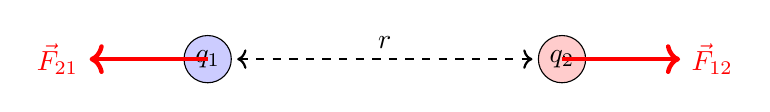
\begin{tikzpicture}[scale=1.5]
        % Charge 1
        \draw[fill=blue!20] (0,0) circle (0.2) node {$q_1$};
        % Charge 2
        \draw[fill=red!20] (3,0) circle (0.2) node {$q_2$};
        
        % Distance line
        \draw[<->, dashed, thick] (0.25,0) -- (2.75,0) node[midway, above] {$r$};
        
        % Force arrows (Repulsion example)
        \draw[->, ultra thick, red] (0,0) -- (-1,0) node[left] {$\vec{F}_{21}$};
        \draw[->, ultra thick, red] (3,0) -- (4,0) node[right] {$\vec{F}_{12}$};

        %\node[below] at (1.5, -0.5) {\textit{Example: Repulsive force between like charges}};
    \end{tikzpicture}
\end {center}
    
\item Forces are equal in magnitude and opposite in direction (Newton's 3rd Law).
\item The force acts along the line joining the two points.


\pagebreak
\item Units and the Permittivity of Vacuum
\item \textbf{Unit of Charge:} The SI unit is the \textbf{Coulomb (C)}. Defined in terms of electric current: $1\,\text{C} = 1\,\text{A} \cdot 1\,\text{s}$.
\item \textbf{Permittivity of Vacuum ($\epsilon_0$):} Coulomb's constant $k$ is often expressed as:
$$ k = \frac{1}{4\pi\epsilon_0} $$
\item \textbf{Value of $\epsilon_0$:}
$$\epsilon_0 \approx 8.854 \times 10^{-12} \, \frac{\text{C}^2}{\text{N}\cdot\text{m}^2} $$
\item This constant represents the capability of a vacuum to permit electric field lines.

\end{itemize}
      
\end{frame}


% ----------------------------------------------------------------------------------------------------------------------------------------

\begin{frame}[fragile,squeeze,allowframebreaks]
\frametitle{The Electrostatic Field}
\begin{itemize}
\setlength{\parskip}{0pt}
\setlength{\itemsep}{4pt}

\item \textbf{Definition:} A region around a charged particle where a force would be exerted on other charged particles.
\item \textbf{Electric Field Strength ($\vec{E}$):} Defined as the force ($F$) per unit positive test charge ($q_0$).
\item \textbf{Equation:} 
$$ \vec{E} = \frac{\vec{F}}{q_0} \quad [\text{Unit: } N/C \text{ or } V/m] $$

\pagebreak
\item \textbf{Electric Field Lines of a Positive Point Charge}
\begin{columns}
\begin{column}{0.5\linewidth}
\vfill
\centering
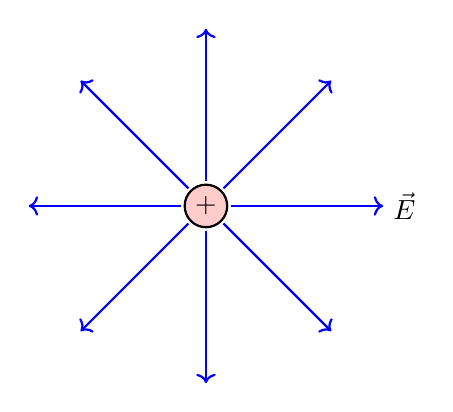
\begin{tikzpicture}[scale=0.9]
% Draw positive charge
\draw[fill=red!20, thick] (0,0) circle (0.3) node {$+$};
% Draw field lines
\foreach \angle in {0,45,90,135,180,225,270,315}
\draw[blue, thick, ->] (\angle:0.35) -- (\angle:2.5);
\node at (2.8,0) {$\vec{E}$};
\end{tikzpicture}
\end{column}
\begin{column}{0.5\linewidth}
\item Electric Field Lines
\begin{itemize}
\item Originate from positive charges, terminate at negative charges.
\item The density of lines represents the field strength.
\item For a \textbf{Point Charge} $Q$, the magnitude is: $E = k \frac{|Q|}{r^2}$
\item The field is spherically symmetric.
\end{itemize}
\end{column}
\end{columns}

\end{itemize}

\end{frame}

% ----------------------------------------------------------------------------------------------------------------------------------------


\begin{frame}[fragile,squeeze,allowframebreaks]
\frametitle{Gauss's Law}
\begin{itemize}

\begin{columns}
  \begin{column}{0.6\linewidth}
  \vfill
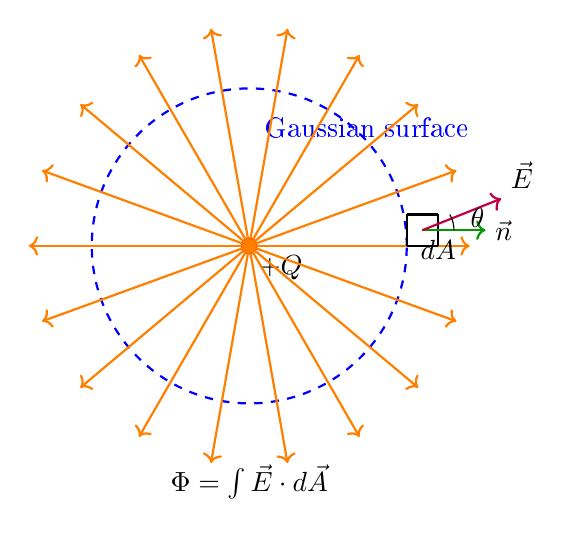
\begin{tikzpicture}[scale=1]

  % Charge
  \filldraw[red] (0,0) circle (0.1);
  \node[below right] at (0,0) {$+Q$};

  % Gaussian surface
  \draw[thick, dashed, blue] (0,0) circle (2);
  \node[blue] at (1.5,1.5) {Gaussian surface};

  % Electric field lines
  \foreach \angle in {0,20,...,340} {
    \draw[->, orange, thick] 
      (0,0) -- ({2.8*cos(\angle)}, {2.8*sin(\angle)});
  }

  % Surface element dA
  \draw[thick] (2,0) -- (2.4,0);
  \draw[thick] (2,0) -- (2,0.4);
  \draw[thick] (2.4,0) -- (2.4,0.4);
  \draw[thick] (2,0.4) -- (2.4,0.4);

  \node[below] at (2.4,0.2) {$dA$};

  % Normal vector
  \draw[->, thick, green!60!black] (2.2,0.2) -- (3,0.2);
  \node[right] at (3,0.2) {$\vec{n}$};

  % Electric field vector at surface
  \draw[->, thick, purple] (2.2,0.2) -- (3.2,0.6);
  \node[above right] at (3.2,0.6) {$\vec{E}$};

  % Angle between E and normal
  \draw (2.6,0.2) arc[start angle=0,end angle=30,radius=0.4];
  \node at (2.9,0.35) {$\theta$};

  % Flux formula
  \node at (0,-3) {$\Phi = \int \vec{E} \cdot d\vec{A}$};

\end{tikzpicture}
\end{column}
\begin{column}{0.4\linewidth}
\item \textbf{Electric Flux ($\Phi_E$):} The measure of the "flow" of the electric field through a surface.
  $$ \Phi_E = \oint_S \vec{E} \cdot d\vec{A} $$
\end{column}
\end{columns}

\pagebreak
\item \textbf{Flux through a Gaussian Surface}
\vskip -10 pt
\begin{columns}
\begin{column}{0.5\linewidth}
    \centering

    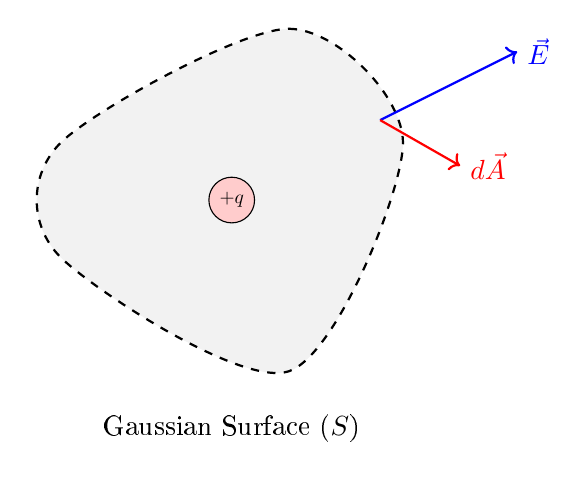
\begin{tikzpicture}[scale=1.45]
        % Draw arbitrary closed surface
        \draw[thick, dashed, fill=gray!10] plot [smooth cycle] coordinates {(0,0) (2,1) (3,0) (2,-2) (0,-1)};
        % Draw charge inside
        \draw[fill=red!20] (1.5,-0.5) circle (0.2) node[scale=0.7] {$+q$};
        % Draw an E-field vector passing through a surface element
        \draw[blue, thick, ->] (2.8,0.2) -- (4,0.8) node[right] {$\vec{E}$};
        \draw[red, thick, ->] (2.8,0.2) -- (3.5, -0.2) node[right] {$d\vec{A}$};
        \node at (1.5, -2.5) {Gaussian Surface ($S$)};
    \end{tikzpicture}

\end{column}
\begin{column}{0.55\linewidth}
\vfill 
\item \textbf{Gauss's Law Statement:} The net electric flux through any closed surface is equal to the net charge enclosed divided by $\varepsilon_0$.
\item Mathematical Form
  $$ \oint_S \vec{E} \cdot d\vec{A} = \frac{Q_{\text{enclosed}}}{\varepsilon_0}, $$ where $d\vec{A}$ is the area vector (perpendicular to the surface).
\item This law is fundamental for calculating fields of symmetric objects (spheres, cylinders, planes).
\end{column}
\end{columns}

\pagebreak
\item Charge Distribution in Conductors with Cavities Why do charges move to the outer surface? Gauss's law argument

\begin{columns}
\begin{column}{0.4\textwidth}

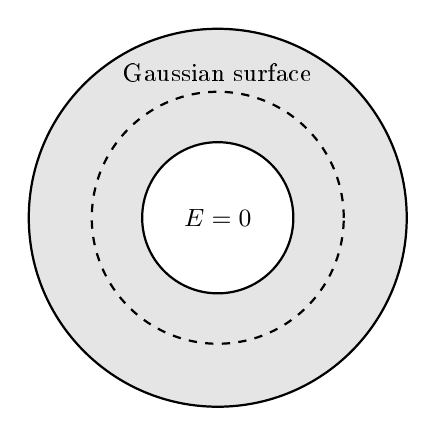
\begin{tikzpicture}[scale=0.8]

% Outer conductor
\fill[gray!20] (0,0) circle (3);

% Cavity
\fill[white] (0,0) circle (1.2);

% Gaussian surface
\draw[dashed, thick] (0,0) circle (2);

% Boundaries
\draw[thick] (0,0) circle (3);
\draw[thick] (0,0) circle (1.2);

\node at (0,2.3) {\small Gaussian surface};
\node at (0,0) {\small $E=0$};

\end{tikzpicture}
\end{column}

\begin{column}{0.6\textwidth}

\textbf{Gauss's law:}
$\oint \mathbf{E} \cdot d\mathbf{A} = \frac{Q_{\text{inside}}}{\varepsilon_0}$

\begin{itemize}
\item Inside the conductor: $\mathbf{E}=0$
\item Therefore the flux is zero.
\item Hence $Q_{\text{inside}}=0$.
\end{itemize}

\textbf{Conclusion:}
\begin{itemize}
\item No net charge can exist inside the conductor.
\item All excess charge must reside on the surface.
\end{itemize}
\end{column}
\end{columns}

\end{itemize}
\end{frame}

% ----------------------------------------------------------------------------------------------------------------------------------------


\begin{frame}
%\frametitle{Minden jó, ha a vége jó}

\vfill
\begin{center}
\textbf{\huge The End}

\bigskip
Thank you for your attention!
\end{center}
\vfill
\textbf{Acknowledgements} Thank you for the course materials for Szilárd~ZSÓKA and Zoltán~VARGA.
\end{frame}

\end{document}
